\chapter{Hierarchical Paragraph Vectors}\label{hierarchical-paragraph-vectors}

\section{Hierarchies and NLP}\label{hierarchies-and-nlp}

Today, there is a vast amount of text available to be used in NLP\@. Many texts (for example articles, websites, books, comments, reviews and messages), are naturally divided into sub-texts (for example chapters, sections, paragraphs and sentences). Furthermore, they are usually also categorized or tagged (for example by authors, publishers, domain names, references, topics and genres).

Consider for example a book about how to learn programming Ruby. This book is divided into multiple chapters, which, in turn, are divided into multiple sections and sentences. Furthermore, this book is found on Amazon in the category ``Programming'', which, in turn, can be found in ``Computers \& Technology'', as can be observed in Figure~\ref{fig:4:book-example}.

Now what do these hierarchies represent? The structure represents concepts and abstractions, which represent potentially useful information. For example, if a person reads multiple articles about the French revolution, they can better predict which words will appear the next article about the French revolution. Thus, if this information can be used to learn the word embeddings, it lends itself for exploitation in the training of word embeddings.

\begin{figure}
	\centering
	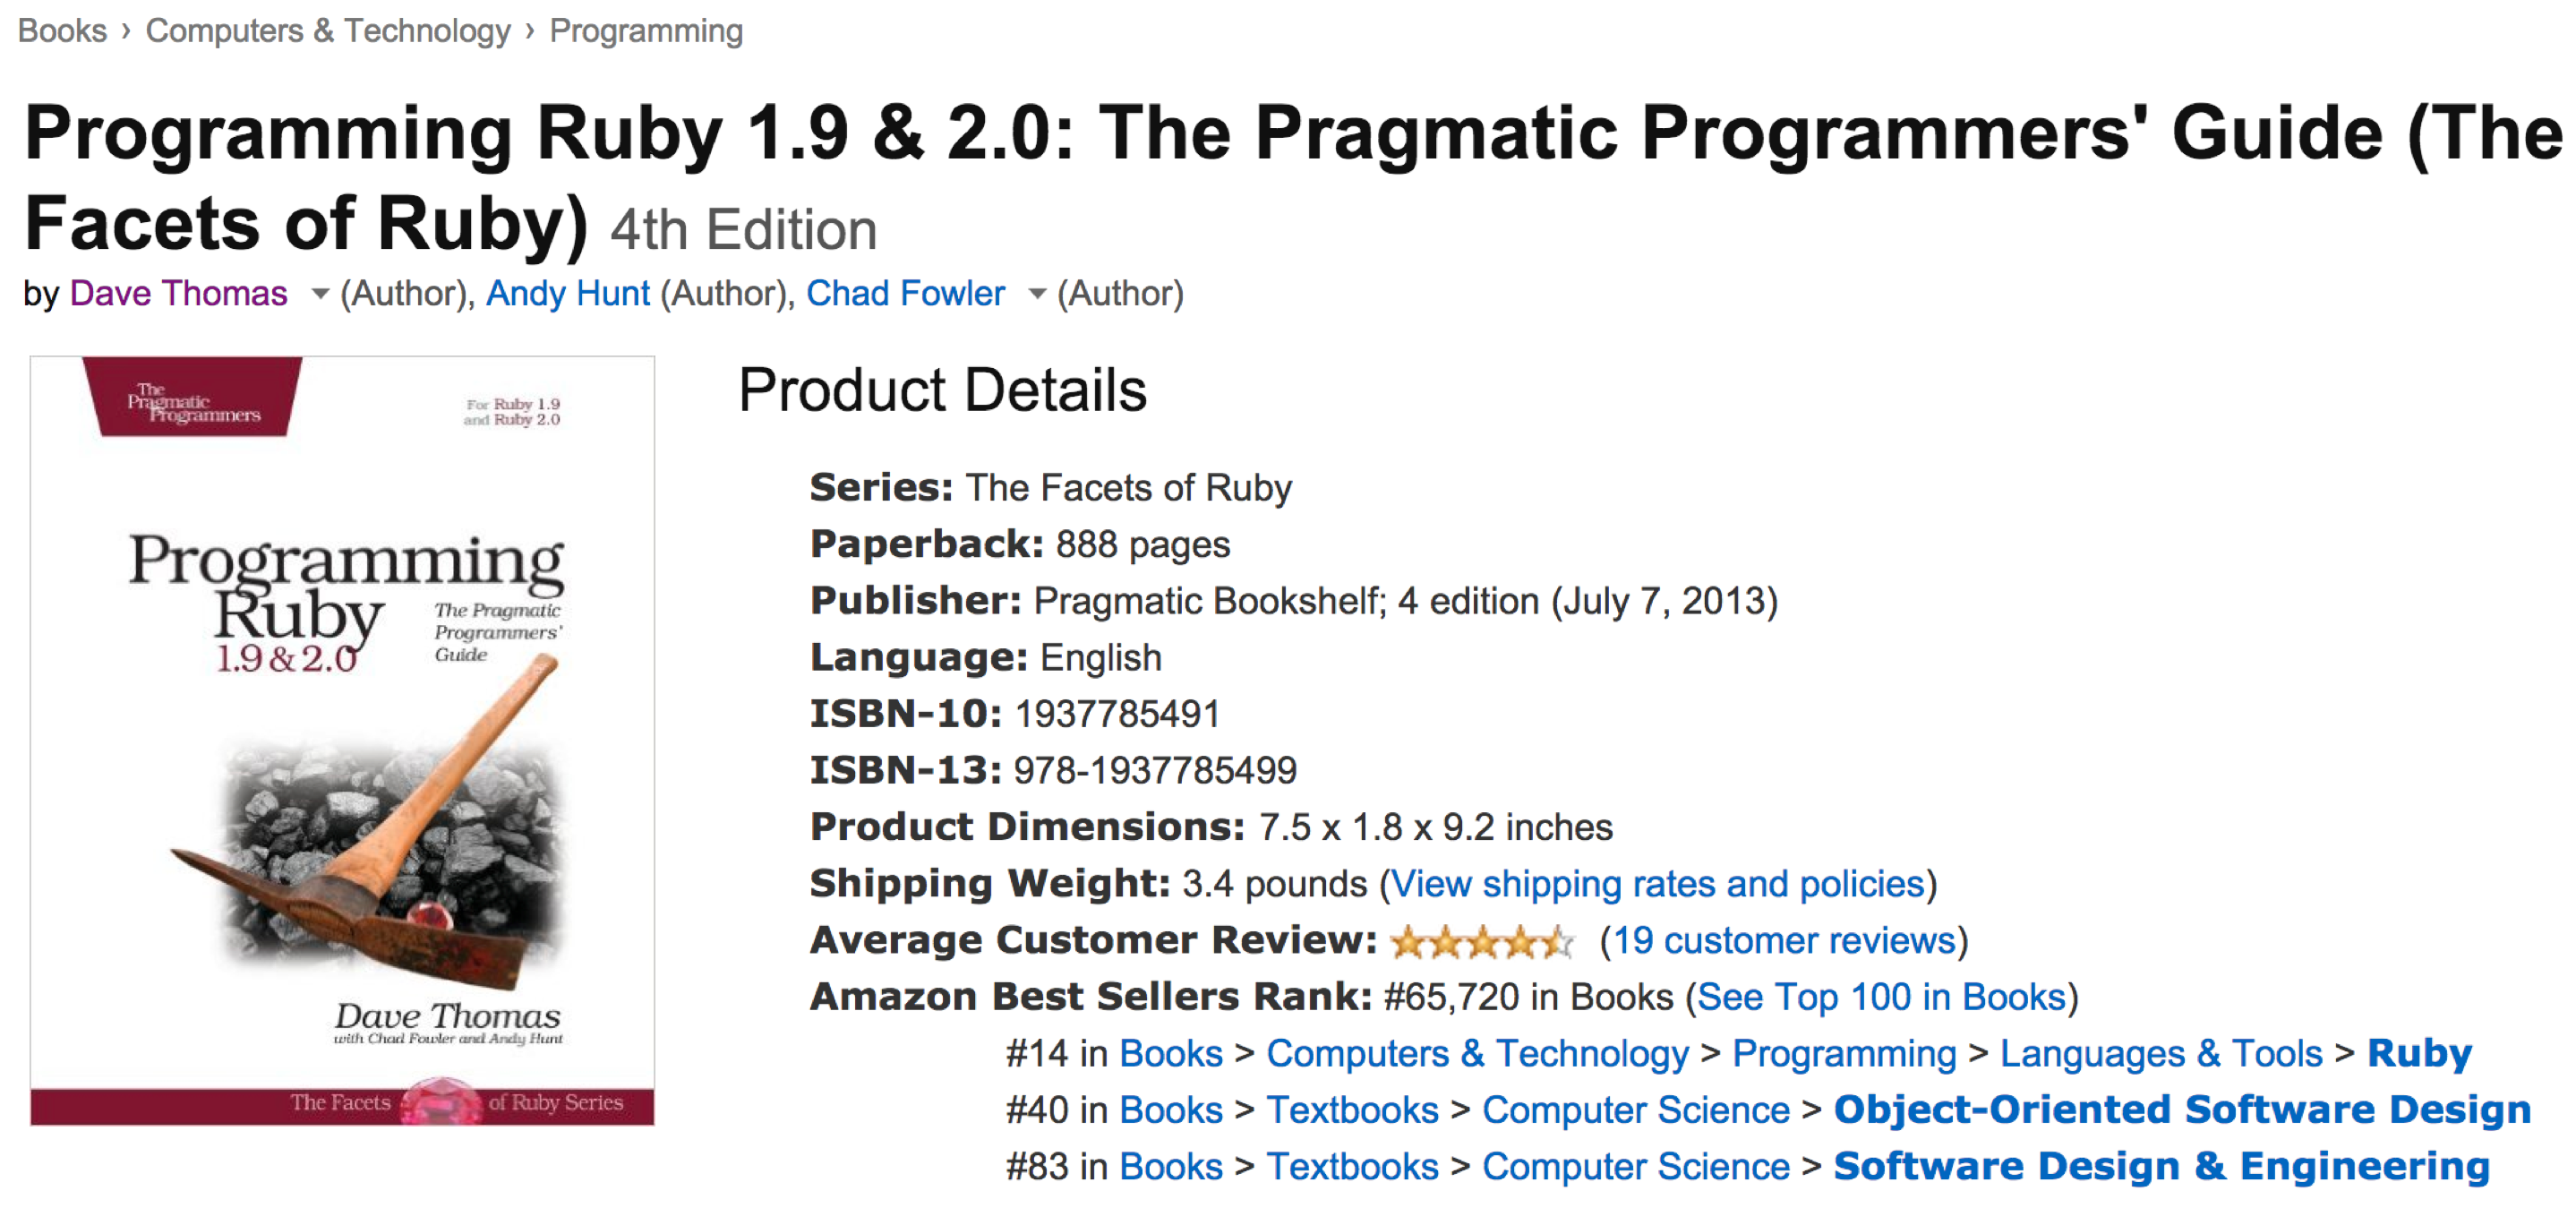
\includegraphics[width=0.9\textwidth]{4hpvs/book-example.png}
	\caption[Caption for LOF]{This book is categorized into ``Programming'' (on the very top of the image), ``Ruby'', ``Object-Oriented Software Design'' and ``Software Design \& Engineering'', which, in turn, can be found in their respective parent category. There are also additional attributes, for example the language of the book and the authors.\footnotemark}
	\label{fig:4:book-example}
\end{figure}

\section{Obtaining Hierarchies}\label{obtaining-hierarchies}

From the perspective of a document, there are potentially two directions in which hierarchies are found. One is ``upwards'', and the other is ``downwards''. Let us define what we mean by that, and how these hierarchies can be obtained.

``Upwards'' refers to hierarchies across multiple documents. As stated above, natural hierarchies are for example author names, publishers, domain names, references, topics or genres. Where available, these can be obtained directly from the data. If this data is not available, it could be generated artificially by standard machine learning methods, for example by Latent Dirichlet Allocation (LDA).

``Downwards'' describes hierarchies to be found within a single document. These could for example be chapters, paragraphs or sentences. These hierarchies are also often available directly through the data, or can be obtained by parsing the text or markup. For example, when an HTML document is given, the HTML tags (for example h1, h2, h3, p, br) can be used to split the text into multiple blocks, and the resulting text blocks can be parsed and split up by sentence.

\footnotetext{Source: \url{http://www.amazon.com/gp/product/1937785491}}

\section{Algorithms}\label{algorithms}

\subsection{HPV-DM}\label{hpv-dm}

HPV-DM builds upon PV-DM\@. Instead of only allowing one paragraph vector per context, it allows multiple hierarchical paragraph vectors for the same context, as can be seen in Figure~\ref{fig:4:hpv-dm}. Additionally, some hierarchical paragraph vectors appear multiple times in different contexts. Similar to the paragraph vectors, the hierarchical paragraph vectors can be thought of as additional memory for the current context, or as additional words which are always present in some context.

\begin{figure}
	\centering
	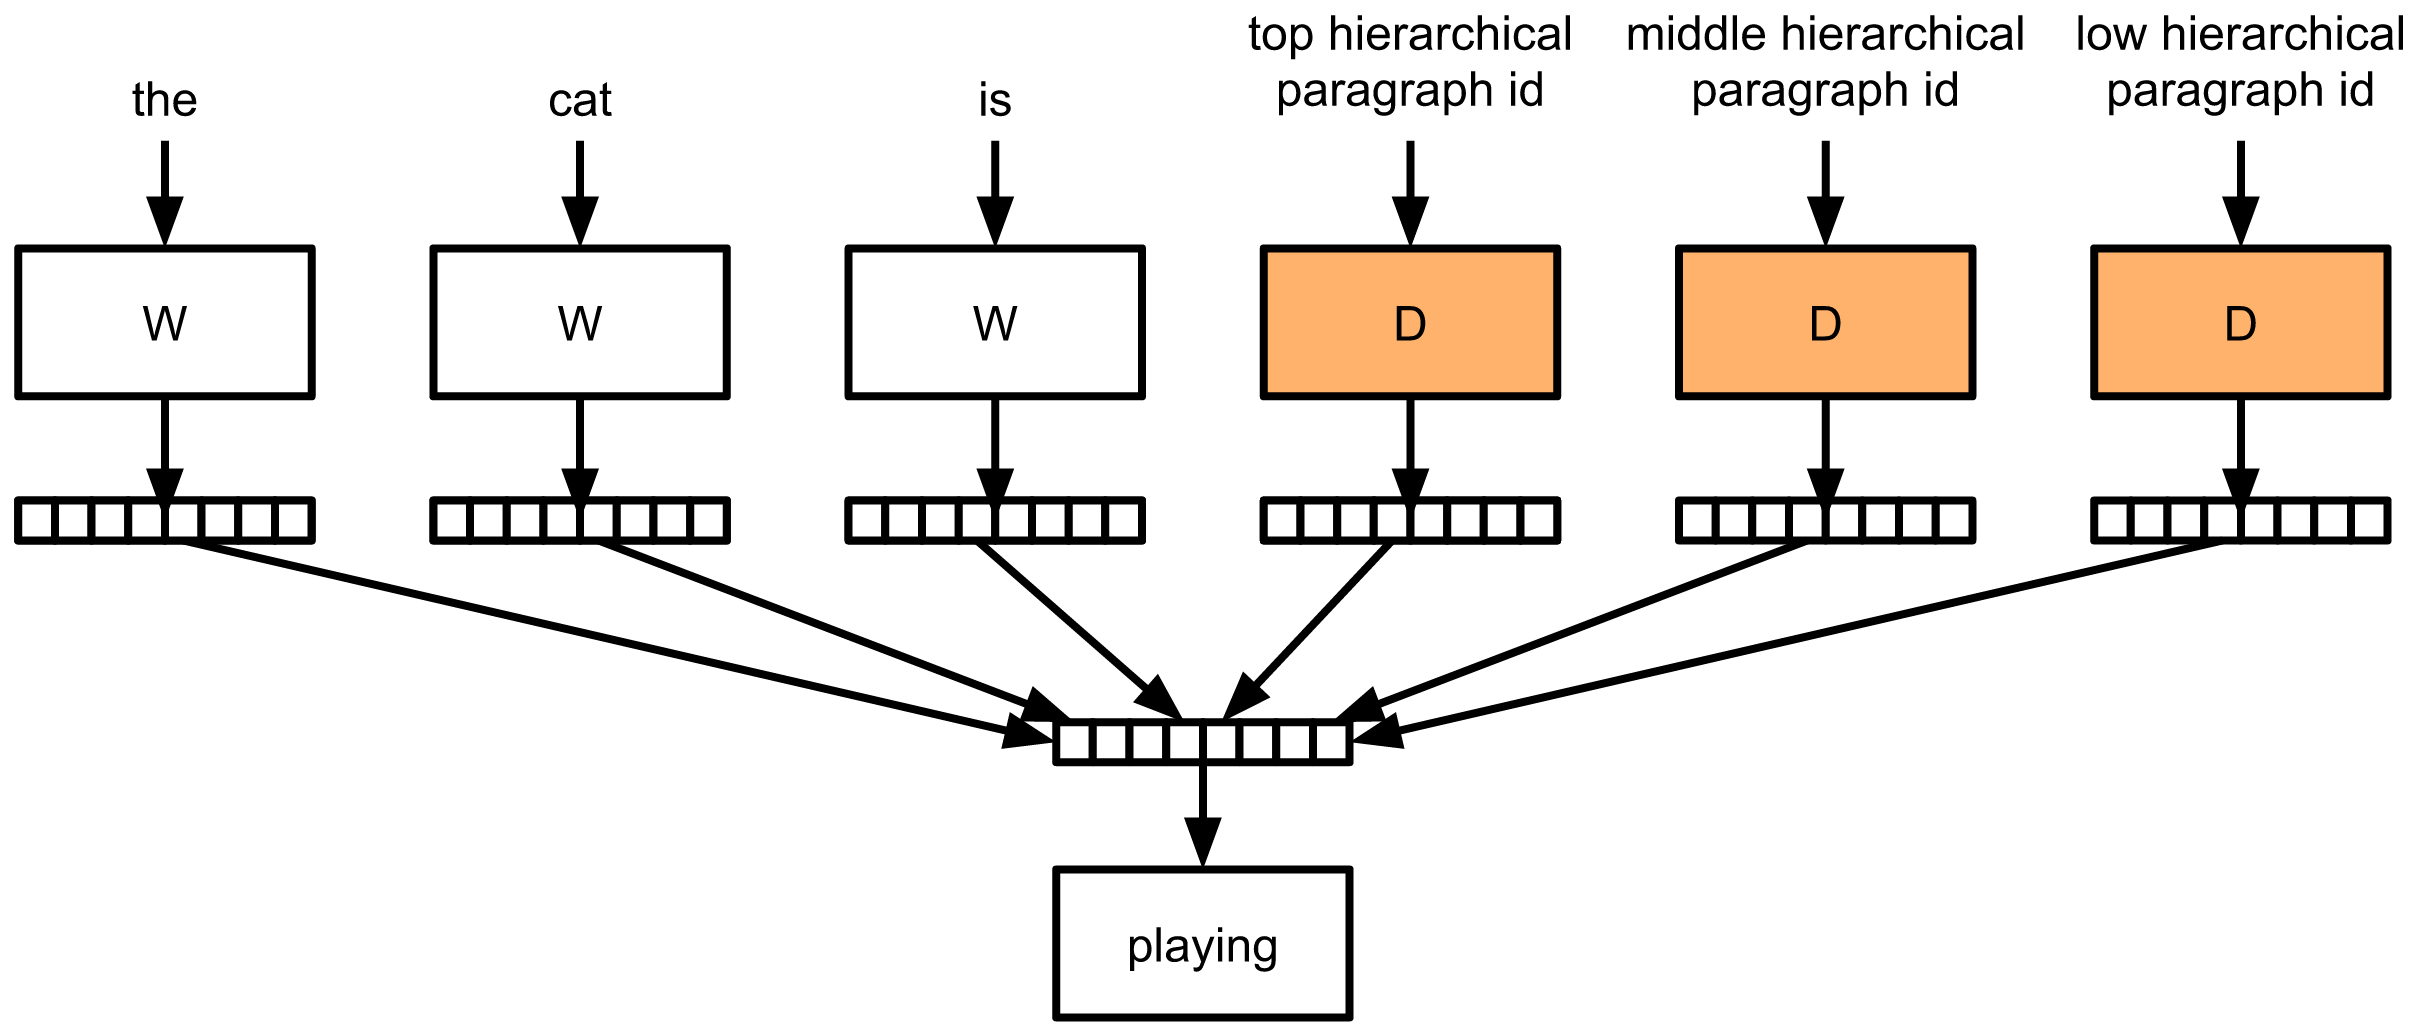
\includegraphics[width=1.0\textwidth]{4hpvs/hpv-dm.png}
	\caption{The architecture of the neural network of HPV-DM\@. Multiple HPVs contribute to the prediction of the word in the context.}
	\label{fig:4:hpv-dm}
\end{figure}

The algorithm works as follows. We split the text into multiple text blocks, according to the hierarchies we want to use. Every item in the hierarchy receives a \emph{unique HPV identifier across the whole dataset}. Next, we add each resulting text block with the HPV annotations as paragraph vectors for training. Then, we train each sentence the same way we would train it with PV-DM, but now each text block has multiple HPVs (paragraph vectors), and each HPV is shared among text blocks which have the same HPV annotation. Therefore, each HPV annotation is expected to contribute to the prediction task. As a bonus, the algorithm generates an embedding for each HPV annotation.

%todo low prio write down the algorithm

For example, when we want to use category (upwards), document (the element for which we would like to have an embedding) and sentence (downwards), we generate, for example, ``CAT-10'' for category \#10, ``DOC-2'' for document \#2, and ``DOC-2-SEN-3'' for sentence \#3 in document \#2. Next, when sentence \#3 in document \#2 belongs to the categories \#10 and \#5, we generate ``CAT-10'', ``CAT-5'', ``DOC-2'' and ``DOC-2-SEN-3'' for this sentence. When we now train the sentences in document \#2, the vector for annotation ``DOC-2'' is shared among the sentences.

\subsection{HPV-DBOW}\label{hpv-dbow}

HPV-DBOW works analogously to the HPV-DM, but it enhances the PV-DBOW algorithm instead of the PV-DM algorithm. For the implementation, the only difference is that we use PV-DBOW instead of PV-DM for training. The neural network architecture is described in Figure~\ref{fig:4:hpv-dbow}. We notice that HPVs in higher hierarchies must support more abstract and general concepts.

\begin{figure}
	\centering
	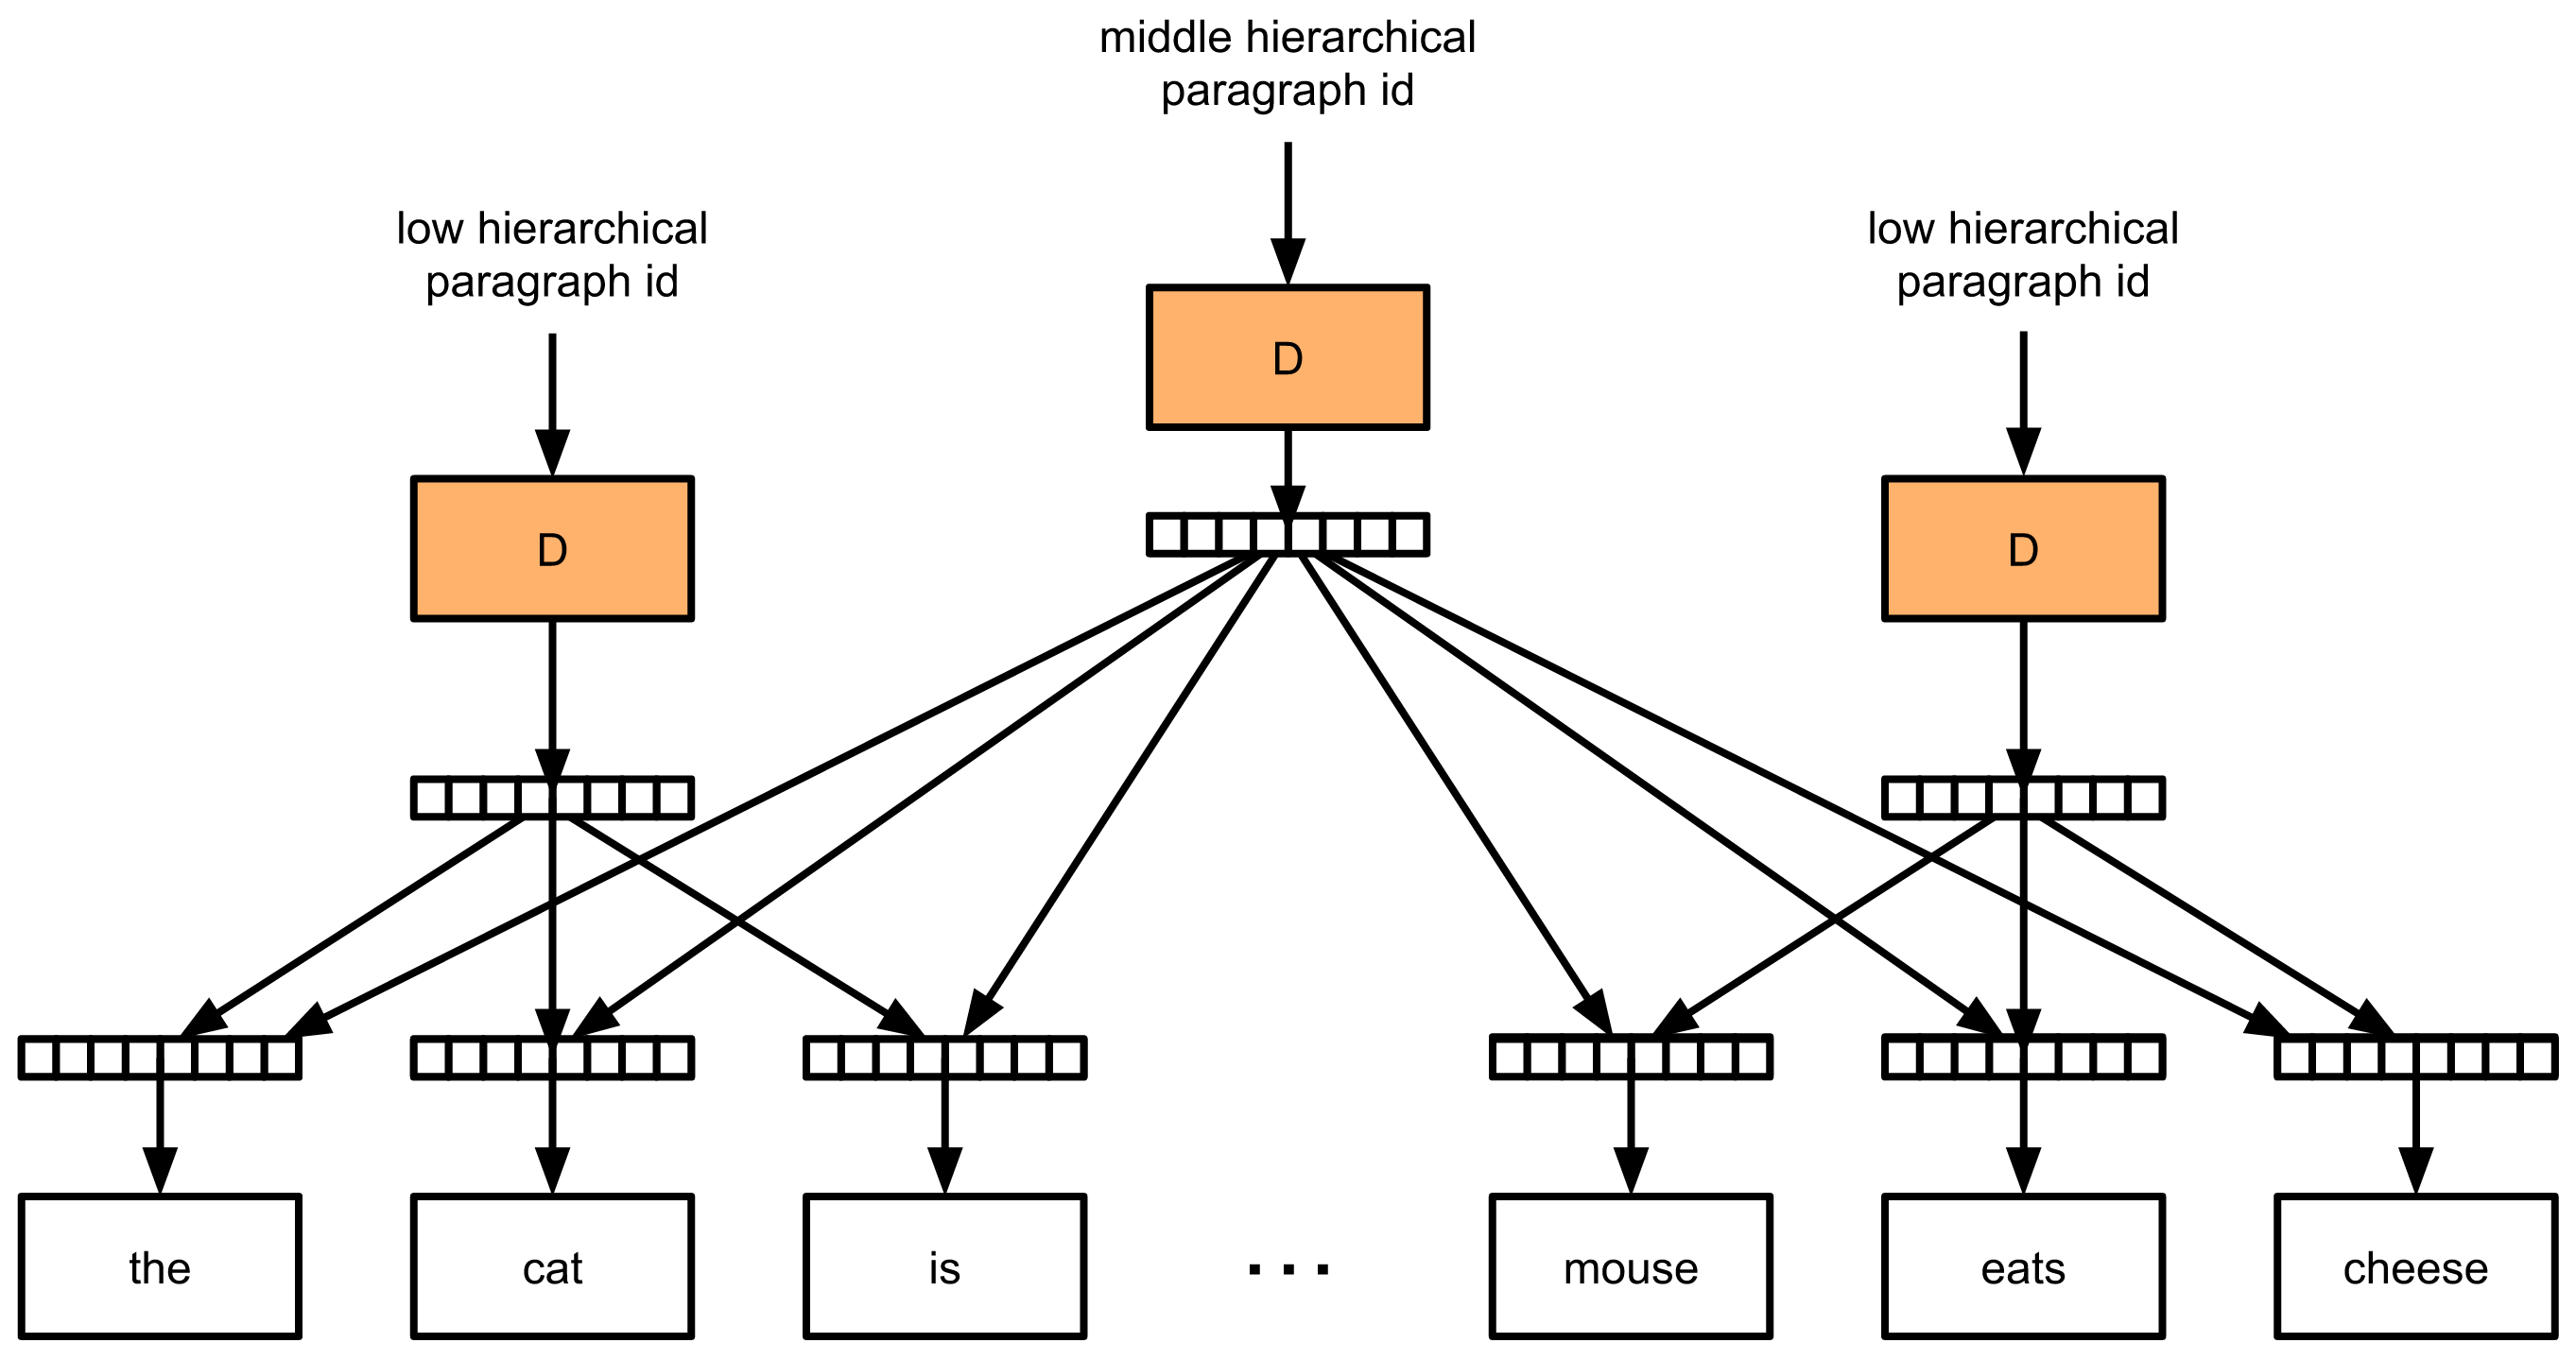
\includegraphics[width=1.0\textwidth]{4hpvs/hpv-dbow.png}
	\caption{The architecture of the neural network of HPV-DBOW\@. Every HPV predicts the context around it. HPVs in higher hierarchies represent more abstract concepts. For example, the lower HPV on the left side captures the behavior of cats, and the lower HPV on the right side captures the behavior of mice. The middle HPV must capture both concepts, which is the behavior of mammals.}
	\label{fig:4:hpv-dbow}
\end{figure}

\subsection{Parameters}\label{parameters}

Because HPV-DM and HPV-DBOW directly extend HP-DM and HP-DBOW respectively, they directly inherit the parameters from these models. However, they introduce a new parameter that dictates which hierarchies should be exploited for learning. While this parameter is limited by the data available, it is important to consider only using the ones which improve the end result, as will be illustrated later.

\section{Resources}\label{4:resources}

When using HPV, we expect to extract additional information at the cost of greater overhead. To estimate how much overhead is introduced, we will discuss how the resources required change when running HPV compared to running PV\@. Therefore, we must first understand how PV influences the resources needed.

Let us start with some definitions. $D$ is the (hierarchical) paragraph vector dimensionality, $E$ is the word vector dimensionality, $G$ is the number of unique different hierarchy elements used, $K$ is the number of paragraph vectors per document, $N$ stands for the number of documents used and $U$ is the vocabulary.

For the Word2vec model, we need to store one word vector per word, which is $E \times \dim(U)$. The paragraph vector models need to additionally store the paragraph vectors, which is $D \times K \times N$ additional memory. Finally, HPV needs to store $D \times G$ additional hierarchical paragraph vectors. Let us write down the formula for the approximate additional memory consumption.
\begin{displaymath}
\frac{D \times G}{E \times \dim(U) +D \times K \times N}
\end{displaymath}

Now, let us briefly discuss what these formulas mean by three typical examples. Let us assume $N=100'000$ documents, $Z=1'000$ average words per document, $D=E=100$ dimensions, $dim(U)=25'000$ vocabulary size, $W=20$ window size, $K=1$ paragraph vectors per document. For the first example, let us assume that we go up in the hierarchy, having 10 topics and 100 subtopics in total. This means $G=110$. In this case, only about 0.009\% additional memory is used. For the second example, assuming that we go downwards, we have 5 sentences per paragraph. This results in $G=50'000$, which means that 143\% additional memory is required. For the third example, let us assume that in addition to the sentences of the second example, there are 4 sub-sentences (in total 200'000) per sentence. Thus, $G=250'000$, which results in 714\% additionally required memory.

Because of the non-trivial optimizations of Word2vec, the runtime implications are more difficult to estimate. Thus, they are not estimated theoretically, but evaluated empirically in Chapter~\ref{experiments} instead.

\section{Research Questions}

As we have seen, HPV introduces additional model complexity. Depending on the number of implemented hierarchy layers, the model gains additional freedom. Can the neural network use this additional complexity to predict better values in the output layer? How many hierarchy layers improve the quality of the word embeddings, and which layers should be chosen? How much overhead is introduced in term of computational complexity and memory usage? Do some layers improve the learning speed of the neural network through the context sharing? We will address these questions in the Chapter~\ref{experiments}.
